\def \MOISEp {$\mathcal{M}OISE^+$}
\def \MOISEpBf {$\mathbf{\mathcal{M}OISE^+}$}

\chapter{Background}
\label{ch:background}

This chapter will explain the theoretical foundation for understanding this work, from the basics of multi-agent systems and modeling these systems to different control architectures used in robotics.

\section{Multi-agents systems}

As presented in \cite{MASSurvey}, Multi-Agent Systems (MAS) is a subfield of Distributed Artificial Intelligence, in which a system is composed of multiple autonomous agents that interact with each other and their environment to achieve individual and collective goals. Agents can communicate, cooperate, and learn with each other, forming complex interactions and using all the gained knowledge to perform actions on the environment. Multi-agent systems (MAS) are well-suited for solving problems in many fields, such as computer science, civil engineering, and electrical engineering. Developing MAS involves tackling a wide range of complex challenges, including agent coordination, learning, and security.

Multi-agent systems (MAS) can be categorized in various ways, depending on the specific characteristics and properties of the system. The four most important types of MAS classifications for this work will be detailed as follows.

The first characteristic of a system is regarding its leadership, a MAS can be either leader-follow or leaderless. A leader-follow system is a system that contains an agent that acts as the leader of the organization, while a leaderless MAS does not. This leader agent is an agent responsible for defining what the other agents should do, by performing task assignments. The leader can be predefined or can be collaboratively chosen by the other agents, besides that it is also possible to have multiple leaders in an organization, which work together to lead the other agents.

The second attribute is the heterogeneity of the MAS. A MAS can be composed of many agents that have different characteristics and functionalities or be composed of agents that have the same features, in the first case the system is categorized as a heterogeneous system, and in the second case as a homogeneous system.

The third characteristic is related to the topology of the MAS. The system topology defines the position and relationship between the agents in the organization, defining, for example, which agents each one can communicate with. This topology can be either static, remaining the same during the MAS execution, or dynamic, changing over time.

Lastly, the fourth attribute regards the mobility of the agents, which specifies if the agents in the system are mobile or static. A static agent always remains in the same position in the environment, while a mobile agent can move around.

\section{\MOISEpBf}

\MOISEp \cite{MOISEp} is a framework for modeling MAS developed by researchers from the University of São Paulo together with researchers from the Ecole Nationale Supérieure des Mines de Saint-Etienne, which extends its predecessor, called MOISE (Model of Organization for multI-agent SystEms) \cite{Moise}. Therefore, to better understand \MOISEp it is first necessary to comprehend the basics concepts of the MOISE model.

MOISE is a framework for designing and developing complex and dynamic organizations for multi-agent systems using an organization-centric point of view. The model provides a structured way of defining an organization so that all the agents work together in a coordinated and efficient manner, this structure is obtained by linking the roles that an agent can play to the plans that need to be executed for the organization to work as a whole. The model is divided into three levels:

\begin{itemize}
    \item \textit{Individual level}: The behavior that needs to be performed for a specific role.
    \item \textit{Social level}: The relationships between the roles.
    \item \textit{Collective level}: The aggregation of roles in large structures.
\end{itemize}

Nevertheless, certain limitations within MOISE required addressing to enhance the framework, such as the lack of the ability to explicitly define global plans for the system within the model. And it was for this reason that the model needed to be extended to the \MOISEp model \cite{MOISEp}. \MOISEp introduces three types of specifications that collectively define the framework: Structural Specification, Functional Specification, and Deontic Specification. These three specifications are essential for defining how the MAS organization works so it can reach its goal.

The \textbf{Structural Specification} delineates the organizational structure, defining the roles that the agents can play, their interrelationships, and group affiliations. This specification allows for the definition of hierarchical relationships, compatibility between roles, role authority, and other relevant characteristics. It also enables the specification of whether one role holds authority over another, the compatibility constraints between roles, and the number of agents that can be assigned to a particular role, among other structural details. An example of a \textbf{Structural Specification} from a MAS can be seen in Figure \ref{fig:moise_ss}.

\begin{figure}
    \centering
    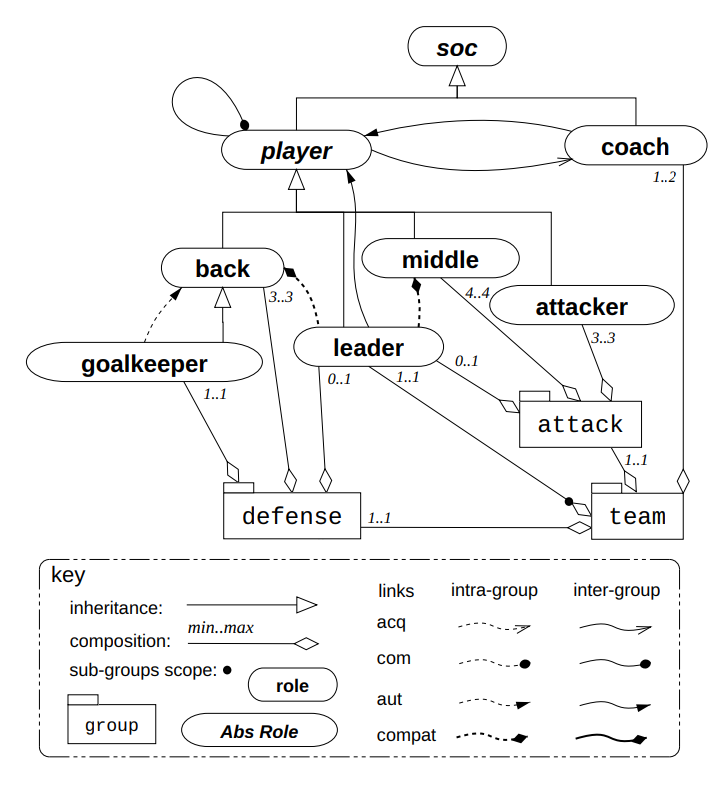
\includegraphics[width=0.75\linewidth]{chapters/background/images/MOISE - SS.png}
    \caption{Structural Specification of a soccer team. Taken from \cite{MOISEp}}
    \label{fig:moise_ss}
\end{figure}

From this example, it is possible to understand the different categories of links between the roles that exist. A link has two attributes, its type, presented in Table \ref{tab:types_of_links_in_moise}, and its scope, which can be intra-group or inter-group. An intra-group link is used to specify that an agent playing the link source role is linked to all agents playing the destination role within the group or any of its sub-groups. Meanwhile, an inter-group link connects despite the groups the agents it connects belongs to.

\def \sourceagent{$a_s$ }
\def \destagent{$a_d$ }

\begin{table}[!htbp]
    \begin{minipage}{\columnwidth}
        \centering
        \begin{tabular}{l l}
            \toprule
            Types         & Meaning                                                        \\
            \midrule
            Acquaintance  & \sourceagent is allowed to have a representation of \destagent \\
            Communication & \sourceagent is allowed to communicate with \destagent         \\
            Authority     & \sourceagent is allowed to have authority over \destagent      \\
            Compatibility & \sourceagent is also allowed to play the destination role      \\
            \bottomrule
        \end{tabular}
        \begin{center}
            \footnotesize
            \emph{Note}: \sourceagent stands for the agent playing the source role of the link \\
            and \destagent stands for the agent playing the destination role. \\
        \end{center}
    \end{minipage}
    \caption{Types of links between the roles in \MOISEp}
    \label{tab:types_of_links_in_moise}
\end{table}

Conversely, the \textbf{Functional Specification} is employed to define a way the goals of the organization can be achieved. It involves defining global plans, a structured way of combining goals, and utilizing a set of global goals to formulate missions. These missions serve as the foundation for the organization's social scheme, and agents within the organization can commit to missions in accordance with the rules defined in the social scheme of how many agents can commit to a specified mission. An example of a social scheme is illustrated in Figure \ref{fig:moise_fs}.

Lastly, the \textbf{Deontic Specification} establishes the relationship between the Structural and Functional Specifications by specifying the permissions and obligations associated with each role in relation to a mission.

\begin{figure}[!h]
    \centering
    \begin{subfigure}{.44\linewidth}
        \centering
        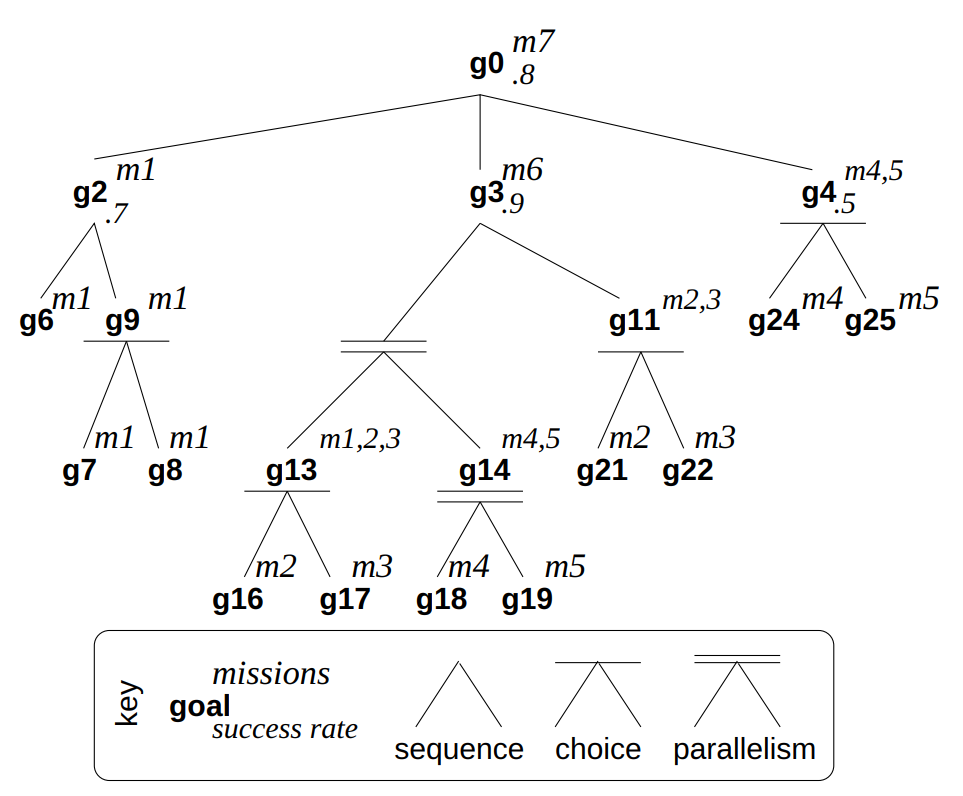
\includegraphics[width=\linewidth]{chapters/background/images/Moise - Social Scheme.png}
    \end{subfigure}
    \hfill
    \begin{subfigure}{.55\linewidth}
        \centering
        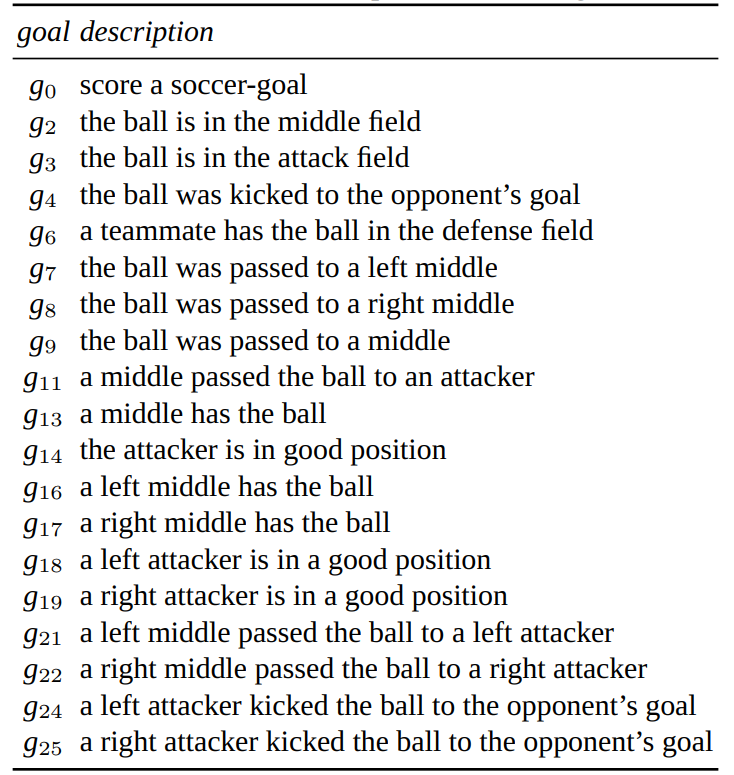
\includegraphics[width=0.8\linewidth]{chapters/background/images/Moise - Goals Descriptions.png}
    \end{subfigure}
    \caption{Example of Social Scheme to score a soccer goal. Taken from \cite{MOISEp}}
    \label{fig:moise_fs}
\end{figure}

\section{Control Architectures}

As defined in \cite{BTsInRobotics2}, a control architecture is a way of encoding a robot's functionality, by defining how a specified task is carried out. A control architecture provides a structured form of defining the intelligence of an agent, facilitating its comprehension, development, and debugging. There are many different types of control architectures that have been developed, each featuring a distinct set of tools, rules, and guidelines for organizing how to control a system.

In this section, two of the most common control architectures in robotics are presented, Finite State Machines (FSM) and Hierarchical Finite State Machines (HFSM). In the next section, the control architecture that is the focus of this work is presented, the Behavior Trees (BT).

\subsection{Finite State Machines}

FSMs are a very common mathematical model of computation, a FSM represents a system which, at any moment in time, can only be in one of a finite number of states. A FSM is defined by a list of states, an initial state, and a set of transition functions that determine how the system transits from one state to another, depending on some inputs, in addition to also being able to have final states of the system. The FSM can be represented as a directed graph, where the states are the nodes and the transitions are the edges. An example of a FSM can be seen in Figure \ref{fig:fsm_example}, where a FSM with three states is depicted, in which $s_1$ is the initial state, $s_3$ is the final one and the transitions between states are triggered by receiving a 1 or a 0.

\begin{figure}[!h]
    \centering
    \begin{tikzpicture}[shorten >=1pt,node distance=2cm,on grid,auto]
        \tikzstyle{every state}=[fill={rgb:black,1;white,10}]

        \node[state,initial]   (s_1)                {$s_1$};
        \node[state]           (s_2) [right of=s_1] {$s_2$};
        \node[state,accepting] (s_3) [right of=s_2] {$s_3$};

        \path[->]
        (s_1) edge [loop above] node {0} (   )
        (s_1) edge [bend left]  node {1} (s_2)
        (s_2) edge [bend left]  node {1} (s_3)
        (s_2) edge [loop above] node {0} (   );
    \end{tikzpicture}
    \caption{Example of a FSM}
    \label{fig:fsm_example}
\end{figure}

As described in \cite{BTsInRobotics}, FSMs are a very intuitive control architecture and can be easily implemented, however, they are not very suitable for describing complex systems. FSMs usually do not scale well, as adding more and more states and transitions to the system, makes it harder to understand and modify. Besides that, FSMs have also a problem regarding maintainability, as adding or removing states can result in re-evaluating numerous transitions and internal states, making FSMs prone to human design errors and impractical for automated design purposes.

\subsection{Hierarchical Finite State Machines}

Hierarchical Finite State Machine (HFSM), also referred to as State Charts, is another type of control architecture that is derived from FSMs. HFSMs are based on the concept of superstates, the idea that a state can contain one or more substates. Thus, in HFSMs there is also the concept of \textit{generalized transitions}, which allow transition from one superstate to another instead of countless transitions between substates, reducing the total number of transitions specified in the system. It is also important to note that, each superstate designates one substate as the starting state, which executes whenever a transition to the superstate occurs. An example of HFSM is illustrated in Figure \ref{fig:hfsm_example}.

\begin{figure}
    \centering
    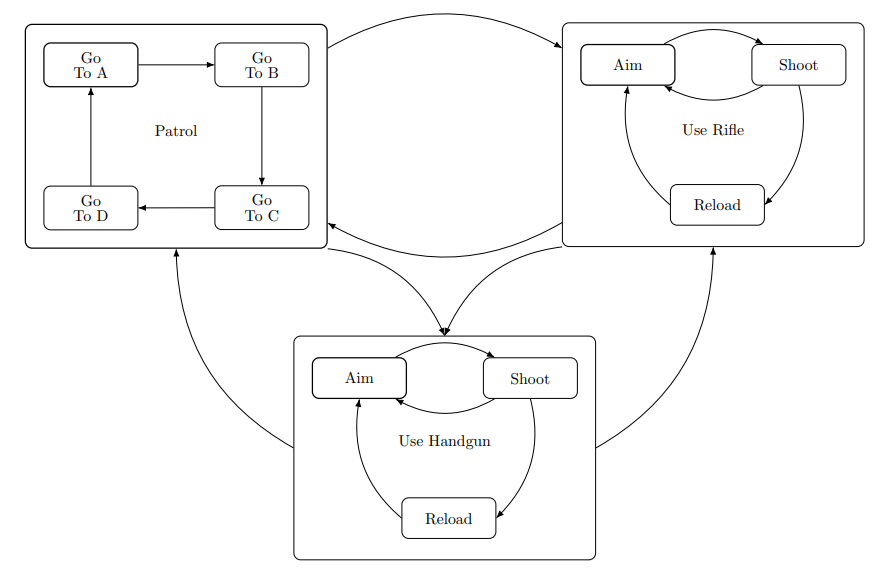
\includegraphics[width=0.75\linewidth]{chapters/background/images/HFSM Example.png}
    \caption{Example of a HFSM controlling a NPC of a combat game. \textit{Patrol}, \textit{Use Rifle}, and \textit{Use Handgun} are superstates. Taken from \cite{BTsInRobotics}}
    \label{fig:hfsm_example}
\end{figure}

As it is possible to observe, HFSMs were developed to address some of the shortcomings of FSMs, trying, for example, to alleviate the problem of the number of transitions in complex systems by the means of using \textit{generalized transitions}. Additionally, this control architecture offers enhanced modularity, allowing tasks to be divided into subtasks, and supports behavior inheritance, enabling a substate to inherit properties from its superstate. However, HFSMs still have some of the same problems as FSMs, such as the difficulty of maintaining and modifying the system, and other problems such as editing the system hierarchy manually.

\section{Behavior Trees}

Behavior Trees (BTs) are a versatile control architecture widely known for their flexibility, modularity, ease of comprehension, and maintainability \cite{BTsInRobotics}. They can be described as a mathematical model that is structured as a directed rooted tree of hierarchical nodes. A BT is composed of two primary types of nodes: the control flow nodes, which are the internal nodes of the tree, and the execution nodes, which are the leaves. By combining various control flow and execution nodes, it is possible to construct a tree that describes an agent's behavior.

As a directed rooted tree, every BT has as its base a root node, which is the one responsible for generating the \textit{tick signal}. This signal is sent from the root throughout the tree until it reaches a leaf node, when this happens, the leaf node is executed and returns a status accordingly, which can be \textit{success}, \textit{failure}, or \textit{running}. The status of the leaf node is propagated back until it returns to the root node, which sends the tick signal all over again throughout the tree, starting a new execution step and continuing the execution of the tree. In a typical BT, the tick signal is propagated from left to right, therefore, a parent node will always tick its leftmost child before ticking the ones from the right.

The internal nodes of the tree, the so called control flow nodes regulate the execution flow of the tree, determining which nodes are executed and the logic of it. The basic control flow nodes in a BT are the fallback node, sequence node, parallel node, and decorator node. On the other hand, execution nodes define commands that the tree should execute. They can be categorized into action nodes and condition nodes. The characteristics and functionalities of these nodes will be delineated in the subsequent subsection.

\subsection{Types of Nodes}

\subsubsection{Root Node}

As previously explained, the root node is the one responsible for sending the tick signal to the whole tree. The node is usually represented as illustrated in Figure \ref{fig:background_root_node}.

\begin{figure}[!h]
    \centering
    \scalebox{.9} {
        \begin{forest}
            [\root, controlflow]
        \end{forest}
    }
    \caption{Representation of a root node}
    \label{fig:background_root_node}
\end{figure}

\subsubsection{Fallback Node}

The \textit{fallback} node, also called \textit{selector}, is a control flow node that iterates through its children from left to right, returning the first occurrence of a child returning either \textit{success} or \textit{running}. If all children return \textit{failure}, the fallback node also returns \textit{failure}. A typical representation of a fallback is a box with the "?" symbol, as can be seen in Figure \ref{fig:background_fallback_node}.

\begin{figure}[!h]
    \centering
    \scalebox{.9} {
        \begin{forest}
            [\reactivefallback, controlflow
                    [{Child 1}, controlflow]
                    [{Child 2}, controlflow]
                    [{...}, minimum height=12mm, minimum width=12mm]
                    [{Child N}, controlflow]
            ]
        \end{forest}
    }
    \caption{Representation of a fallback node}
    \label{fig:background_fallback_node}
\end{figure}

\subsubsection{Sequence Node}

The \textit{sequence} node is also a control flow node that iterates through its children from left to right, however, this node returns \textit{success} only if all of its children return \textit{success} as well, otherwise, it returns \textit{running} or \textit{failure}, depending on its child status. The sequence node is usually represented as a box with the "$\rightarrow$" symbol, as illustrated in Figure \ref{fig:background_sequence_node}.

\begin{figure}[!h]
    \centering
    \scalebox{.9} {
        \begin{forest}
            [\reactivesequence, controlflow
                    [{Child 1}, controlflow]
                    [{Child 2}, controlflow]
                    [{...}, minimum height=12mm, minimum width=12mm]
                    [{Child N}, controlflow]
            ]
        \end{forest}
    }
    \caption{Representation of sequence node}
    \label{fig:background_sequence_node}
\end{figure}

\subsubsection{Parallel Node}

The parallel node simultaneously ticks all of its children and returns \textit{success} if a specified number, M, of its N children return \textit{success}. It returns \textit{failure} if $N - M + 1$ of its children return \textit{failure}, and it returns \textit{running} otherwise. A representation of the use of a parallel node is depicted in Figure \ref{fig:background_parallel_node}, showing that the node is commonly represented using the "$\rightrightarrows$" symbol.

\begin{figure}[!h]
    \centering
    \scalebox{.9} {
        \begin{forest}
            [\parallel, controlflow
                    [{Child 1}, controlflow]
                    [{Child 2}, controlflow]
                    [{...}, minimum height=12mm, minimum width=12mm]
                    [{Child N}, controlflow]
            ]
        \end{forest}
    }
    \caption{Representation of a parallel node}
    \label{fig:background_parallel_node}
\end{figure}

\subsubsection{Decorator Nodes}

Decorator nodes are a special type of control flow node that transforms the result received from its child, depending on a specified policy $\mathbf{\delta}$. The policies of a decorator node can vary greatly, for example, it is possible to use a decorator to invert its child's status, as well as to execute its child a certain number of times. Decorators are represented as rhombus-shaped nodes, with their policy indicated inside, as illustrated in Figure \ref{fig:background_decorator_node}.

\begin{figure}[!h]
    \centering
    \scalebox{0.9} {
        \begin{forest}
            [$\mathbf{\delta}$, decorator
                    [{Child}, controlflow]
            ]
        \end{forest}
    }
    \caption{Representation of a decorator node with policy $\mathbf{\delta}$}
    \label{fig:background_decorator_node}
\end{figure}

\subsubsection{Action Nodes}

The action nodes, represented in Figure \ref{fig:background_action_node}, are a type of execution node, which, as its name implies, perform an action. After being ticked, if the node needs more time to complete its action, it returns the status \textit{running} to its parent, if the action finished successfully, it returns \textit{success}, otherwise, returns \textit{failure}.

\begin{figure}[!h]
    \centering
    \scalebox{.9} {
        \begin{forest}
            [Action, action]
        \end{forest}
    }
    \caption{Representation of an action node}
    \label{fig:background_action_node}
\end{figure}

\subsubsection{Condition Nodes}

The condition nodes, depicted in Figure \ref{fig:background_condition_node}, are used to check propositions. In case the proposition is true, the node returns \textit{success}, otherwise returns \textit{failure}.

\begin{figure}[!h]
    \centering
    \scalebox{.9} {
        \begin{forest}
            [Condition, condition]
        \end{forest}
    }
    \caption{Representation of a condition node}
    \label{fig:background_condition_node}
\end{figure}

\subsubsection{Subtree Nodes}

In addition to the aforementioned nodes, an essential concept in BT design is that of subtrees. When building large-scale trees, it is very useful to be able to divide the tree into smaller parts, creating small modules that are independent of each other, simplifying the development of the overall system. This can be achieved using subtrees, which can be used as components to be incorporated into a larger tree. When the main tree ticks a subtree, the root node of the subtree ticks its children, as if all nodes of the subtree were included in the parent tree. The representation of a subtree is sown in Figure \ref{fig:background_subtree_node}.

\begin{figure}[!h]
    \centering
    \scalebox{.9} {
        \begin{forest}
            [{Subtree}, subtree]
        \end{forest}
    }
    \caption{Representation of a subtree node}
    \label{fig:background_subtree_node}
\end{figure}

\subsection{Reactivity}

Another very important characteristic of BTs is their ability to show reactive and non-reactive behaviors. Reactive behaviors are defined through nodes without memory, that is, every time the node is ticked, it restarts all the execution of its children, allowing the tree to respond faster to changes. On the other hand, non-reactive nodes are denoted as nodes with memory, as these nodes store the statuses of the children that have already been executed. They assume that the statuses of the previously executed children will remain unchanged and proceed to tick the next child that hasn't been ticked yet. This allows for efficient execution and avoids re-evaluating the statuses of already executed children.

This reactivity of the trees is more related to the control flow nodes, more specifically to the sequence and fallback nodes. The difference between the behavior of sequence and fallback nodes regarding their reactivity is presented in Tables \ref{tab:sequence_reactivity} and \ref{tab:fallback_reactivity}, respectively.

\begin{table}[h]
    \centering
    \begin{tabular}{c c c}
        \toprule
        Type of Sequence & Child returns \textit{running} & Child returns \textit{failure} \\
        \midrule
        Reactive         & Restart from first child       & Restart from first child       \\
        Non-reactive     & Tick running child again       & Tick failed child again        \\
        \bottomrule
    \end{tabular}
    \caption{Behavior of reactive and non-reactive sequence nodes when ticked}
    \label{tab:sequence_reactivity}
\end{table}

\begin{table}[h]
    \centering
    \begin{tabular}{c c}
        \toprule
        Type of Fallback & Child returns \textit{running} \\
        \midrule
        Reactive         & Restart from first child       \\
        Non-reactive     & Tick running child again       \\
        \bottomrule
    \end{tabular}
    \caption{Behavior of reactive and non-reactive fallback nodes when ticked}
    \label{tab:fallback_reactivity}
\end{table}

To differentiate the nodes with and without memory, in \cite{BTsInRobotics}, the nodes with memory are marked with the symbol "*", that is, a sequence node with memory is identified by "$\rightarrow^*$", while a fallback node is represented by "$?^*$", as depicted in Figure \ref{fig:background_non_reactive_nodes}.

\begin{figure}[!h]
    \centering
    \begin{subfigure}[b]{.49\linewidth}
        \centering
        \scalebox{1.0} {
            \begin{forest}
                [\sequence, controlflow]
            \end{forest}
        }
        \caption{Non-reactive sequence}
    \end{subfigure}
    \hfill
    \begin{subfigure}[b]{.49\linewidth}
        \centering
        \scalebox{1.0} {
            \begin{forest}
                [\fallback, controlflow]
            \end{forest}
        }
        \caption{Non-reactive fallback}
    \end{subfigure}
    \caption{Representation of non-reactive nodes}
    \label{fig:background_non_reactive_nodes}
\end{figure}

\subsection{Advantages and Disadvantages}

According to \cite{BTsInRobotics}, Behavior Trees (BTs) offer several advantageous characteristics. One notable advantage is their modularity, allowing for easy rearrangement of system blocks and simplifying the subdivision of complex systems. Additionally, the building blocks of BTs can be reused, facilitating the development of large systems. The hierarchical organization of BTs enhances their analysis and understanding, and their human readability is also noteworthy. Another advantage is their ability to exhibit reactive behaviors, enabling quick and efficient responses to events. Lastly, BTs are highly expressive, capable of encoding various behaviors and generalizing numerous control architectures.

However, BTs also present some disadvantages, for example, the fact that compared to FSMs and HFSMs, they are much less mature, although there are already many new technologies related to BTs. Besides that, implementing a BT engine is a complex task, while a FSM can be implemented with a switch statement, however, this problem can be mitigated using already implemented frameworks for developing BTs. Finally, it is important to note that working with BTs requires a shift in mindset compared to FSMs. In BTs, the concept of states, commonly found in FSMs, is not typically used. Instead, the focus is on the hierarchical structure and the flow of execution within the tree. While BTs are generally easier to understand, it is important to approach them with a different perspective.

\section{Blackboard}

A blackboard \cite{BlackboardDesignPattern} is a design pattern in software engineering used when separated processes need to work together in order to make collective decisions. Blackboards are basically a shared memory space or data structure that allows different modules of a system to exchange information. They serve as a central repository where data, variables, and states can be stored and accessed by various parts of the system. Blackboards are very commonly used in the context of control architectures, enabling the exchange of data between the different modules of the system, for example, in the case of BTs, share the output of one node to another node.
